\chapter{Genomic sequence tools}
\label{gst}
The Genomic Sequence subset works directly with the DNA sequences, without any standard format. These tools allow data extraction, summarising and some mathematical operations over the files. Usually, these are used in the pipeline as complementary tools. Currently, genomic sequence tools, for analysis and manipulation, available are:
\begin{enumerate}

\item \texttt{gto\char`_genomic\char`_gen\char`_random\char`_dna}: to generate a synthetic DNA.

\item \texttt{gto\char`_genomic\char`_rand\char`_seq\char`_extra\char`_chars}: to substitute in a DNA sequence the outside ACGT chars by random ACGT symbols.

\item \texttt{gto\char`_genomic\char`_dna\char`_mutate}: to create a synthetic mutation of a sequence file given specific rates of mutations, deletions and additions.

\item \texttt{gto\char`_genomic\char`_extract}: to extract sequences from a sequence file, whose range is defined by the user in the parameters.

\item \texttt{gto\char`_genomic\char`_period}: to calculate the best order depth of a sequence, using FCMs.

\item \texttt{gto\char`_genomic\char`_count\char`_bases}: to count the number of bases in a sequence, FASTA or FASTQ files.

\item \texttt{gto\char`_genomic\char`_compressor}: to compress and decompress genomic sequences for storage purposes (also under the alias gto\char`_geco).

\item \texttt{gto\char`_genomic\char`_complement}: to replace the ACGT bases with their complements in a DNA sequence.

\item \texttt{gto\char`_genomic\char`_reverse}: to reverse the ACGT bases order for each read in a sequence file (also under the alias gto\char`_reverse).

\item \texttt{gto\char`_genomic\char`_variation\char`_map}: this tool is an alias to gto\char`_fastq\char`_variation\char`_map tool. Please check the documentation of this tool in the FASTQ tools section. 

\item \texttt{gto\char`_genomic\char`_variation\char`_filter}: this tool is an alias to gto\char`_fastq\char`_variation\char`_filter tool. Please check the documentation of this tool in the FASTQ tools section. 

\item \texttt{gto\char`_genomic\char`_variation\char`_visual}: this tool is an alias to gto\char`_fastq\char`_variation\char`_visual tool. Please check the documentation of this tool in the FASTQ tools section. 

\end{enumerate}

\section{Program gto\char`_genomic\char`_gen\char`_random\char`_dna}
The \texttt{gto\char`_genomic\char`_gen\char`_random\char`_dna} generates a synthetic DNA.\\
For help type:
\begin{lstlisting}
./gto_genomic_gen_random_dna -h
\end{lstlisting}
In the following subsections, we explain the input and output parameters.

\subsection*{Input parameters}

The \texttt{gto\char`_genomic\char`_gen\char`_random\char`_dna} program needs one stream for the computation, namely the output standard.\\
The attribution is given according to:
\begin{lstlisting}
Usage: ./gto_genomic_gen_random_dna [options] [[--] args]
   or: ./gto_genomic_gen_random_dna [options]

It generates a synthetic DNA.

    -h, --help                show this help message and exit

Basic options
    > output.seq              Output synthetic DNA sequence (stdout)

Optional
    -s, --seed=<int>          Starting point to the random generator (Default 0)
    -n, --nSymbols=<int>      Number of symbols generated (Default 100)
    -f, --frequency=<str>     The frequency of each base. It should be represented 
    						  in the following format: <fa,fc,fg,ft>.

Example: ./gto_genomic_gen_random_dna -s <seed> -n <nsybomls> -f <fa,fc,fg,ft> > output.seq
\end{lstlisting}

\subsection*{Output}
The output of the \texttt{gto\char`_genomic\char`_gen\char`_random\char`_dna} program is a sequence group file with the synthetic DNA.\\
Using 1 as seed value and 400 as the number of symbols, an output example of this is:
\begin{lstlisting}
TCTTTACTCGCGCGTTGGAGAAATACAATAGTGCGGCTCTGTCTCCTTATGAAGTCAACAATTTCGCTGGGACTTGCGGC
TCTTTACTCGCGCGTTGGAGAAATACAATAGTGCGGCTCTGTCTCCTTATGAAGTCAACAATTTCGCTGGGACTTGCGGC
GACTTCATCGTGGTCTCTGTCATTATGCGCTCCAACGCATAACTTTGCGCCAGAAGATAGATAGAATGGTGTAAGAAACT
GTAATATATATAATGAACTTCGGCGAGTCTGTGGAGTTTTTGTTGCATTAGAGAGCCAAGAGGTCGGACGTCCTCACGTA
GCCCGAGACGGGCAGGGCGATGGCGACTGAACGGGCTCCATATCACTTTGAGCTTTTATGCTTTCGACTCCTCCAGGAGC
TGAACAACCTTGTTCCCGGCAAAGCCCACTGCGTCATGGAGCTCACGGTCTACATTCATGACTGACTAACCGTAAACTGC
\end{lstlisting}

\section{Program gto\char`_genomic\char`_rand\char`_seq\char`_extra\char`_chars}
The \texttt{gto\char`_genomic\char`_rand\char`_seq\char`_extra\char`_chars} substitutes, in the DNA sequence, the outside ACGT chars by random ACGT symbols. It works in sequence file formats.\\
For help type:
\begin{lstlisting}
./gto_genomic_rand_seq_extra_chars -h
\end{lstlisting}
In the following subsections, we explain the input and output parameter.

\subsection*{Input parameters}

The \texttt{gto\char`_genomic\char`_rand\char`_seq\char`_extra\char`_chars} program needs two streams for the computation, namely the input and output standard. The input stream is a sequence file.\\
The attribution is given according to:
\begin{lstlisting}
Usage: ./gto_genomic_rand_seq_extra_chars [options] [[--] args]
   or: ./gto_genomic_rand_seq_extra_chars [options]

It substitues in the DNA sequence the outside ACGT chars by random ACGT symbols.
It works in sequence file formats


    -h, --help        show this help message and exit

Basic options
    < input.seq       Input sequence file (stdin)
    > output.seq      Output sequence file (stdout)

Example: ./gto_genomic_rand_seq_extra_chars < input.seq > output.seq
\end{lstlisting}
An example of such an input file is:
\begin{lstlisting}
ANAAGACGNNNTCCTGCTGCTGCTGCTCTCCGGGGCCACGGCCCTGGAGGGTCCACCGCTGCCCTGCTGCCATTGTCCCC
NNCCCCACCTAAGGAAAAGCAGCCTCCTGACTTTCCTCGCTTGGGCCGAGACAGCGAGCATATGCAGGAAGCGGCAGGAA
GTGGTTTGAGTGGACCTCCGGGCCCCNNNNNGGAGAGGAAGCTCGGGAGNGTNNNGGCCAGGCGGCAGNNNNCCAGTGCC
GCGAATCCGCGCGCCGGGACAGAATCTCCTGCAAAGCCCTGCAGGAACTTCTTCTGGAAGACCTTCTCCACCCCCCCAGC
TANNNNCTCACCCATGAATGCTCACGCAAGTTTAATTACAGACCTGAAACAAGATGCCATTGTCCCCCGGCCTCCTGCTG
CTGCTGCTCTCCGGGGCCACGGCCACCGCTGCCCTGCCCCTGGAGGGTGGCCCCACCGGCCGAGACAGCGAGCATATGCA
GGAAGCGGCAGGAATAAGNNNAAGCAGCCTCCTGACTTTCCTCGCTTGNNNNTTTGAGTGGACCTCCCAGGCCAGTGCCG
GGCCCCTCATAGGAGAGGAAGCTCGGGAGGTGGCCAGGCGGCAGGAAGGCGCACCCCCCCAGCAATCCGCGCGCCGGGAC
AGAATGCCCTGCAGGAACTTCTTCTGGAAGACCTTCTCCTCCTGCAAATAAAACCTCACCCATGAATGCTCACGCAAGTT
NNATTACNNNCCTGNN
\end{lstlisting}

\subsection*{Output}
The output of the \texttt{gto\char`_genomic\char`_rand\char`_seq\char`_extra\char`_chars} program is a sequence file.\\
Using the input above, an output example of this is:
\begin{lstlisting}
ATAAGACGGCTTCCTGCTGCTGCTGCTCTCCGGGGCCACGGCCCTGGAGGGTCCACCGCTGCCCTGCTGCCATTGTCCCC
CTCCCCACCTAAGGAAAAGCAGCCTCCTGACTTTCCTCGCTTGGGCCGAGACAGCGAGCATATGCAGGAAGCGGCAGGAA
GTGGTTTGAGTGGACCTCCGGGCCCCGACCGGGAGAGGAAGCTCGGGAGTGTGTTGGCCAGGCGGCAGGAGACCAGTGCC
GCGAATCCGCGCGCCGGGACAGAATCTCCTGCAAAGCCCTGCAGGAACTTCTTCTGGAAGACCTTCTCCACCCCCCCAGC
TAATATCTCACCCATGAATGCTCACGCAAGTTTAATTACAGACCTGAAACAAGATGCCATTGTCCCCCGGCCTCCTGCTG
CTGCTGCTCTCCGGGGCCACGGCCACCGCTGCCCTGCCCCTGGAGGGTGGCCCCACCGGCCGAGACAGCGAGCATATGCA
GGAAGCGGCAGGAATAAGCGGAAGCAGCCTCCTGACTTTCCTCGCTTGGTTTTTTGAGTGGACCTCCCAGGCCAGTGCCG
GGCCCCTCATAGGAGAGGAAGCTCGGGAGGTGGCCAGGCGGCAGGAAGGCGCACCCCCCCAGCAATCCGCGCGCCGGGAC
AGAATGCCCTGCAGGAACTTCTTCTGGAAGACCTTCTCCTCCTGCAAATAAAACCTCACCCATGAATGCTCACGCAAGTT
CGATTACGGCCCTGTC
\end{lstlisting}
\section{Program gto\char`_genomic\char`_dna\char`_mutate}
The \texttt{gto\char`_genomic\char`_dna\char`_mutate} creates a synthetic mutation of a sequence file given specific rates of mutations, deletions and additions. All these parameters are defined by the user, and are optional.\\
For help type:
\begin{lstlisting}
./gto_genomic_dna_mutate -h
\end{lstlisting}
In the following subsections, we explain the input and output parameters.

\subsection*{Input parameters}

The \texttt{gto\char`_genomic\char`_dna\char`_mutate} program needs two streams for the computation, namely the input and output standard. However, optional settings can be supplied too, such as the starting point to the random generator, and the edition, deletion and insertion rates. The user can also choose to use the ACGTN alphabet in the synthetic mutation. The input stream is a sequence file.\\
The attribution is given according to:
\begin{lstlisting}
Usage: ./gto_genomic_dna_mutate [options] [[--] args]
   or: ./gto_genomic_dna_mutate [options]

Creates a synthetic mutation of a sequence file given specific rates of mutations, 
deletions and additions

    -h, --help                    show this help message and exit

Basic options
    < input.seq                   Input sequence file (stdin)
    > output.seq                  Output sequence file (stdout)

Optional
    -s, --seed=<int>              Starting point to the random generator
    -m, --mutation-rate=<dbl>     Defines the mutation rate (default 0.0)
    -d, --deletion-rate=<dbl>     Defines the deletion rate (default 0.0)
    -i, --insertion-rate=<dbl>    Defines the insertion rate (default 0.0)
    -a, --ACGTN-alphabet          When active, the application uses the ACGTN alphabet

Example: ./gto_genomic_dna_mutate -s <seed> -m <mutation rate> -d <deletion rate> -i 
<insertion rate> -a < input.seq > output.seq
\end{lstlisting}
An example of such an input file is:
\begin{lstlisting}
TCTTTACTCGCGCGTTGGAGAAATACAATAGTGCGGCTCTGTCTCCTTATGAAGTCAACAATTTCGCTGGGACTTGCGGC
TCTTTACTCGCGCGTTGGAGAAATACAATAGTGCGGCTCTGTCTCCTTATGAAGTCAACAATTTCGCTGGGACTTGCGGC
GACTTCATCGTGGTCTCTGTCATTATGCGCTCCAACGCATAACTTTGCGCCAGAAGATAGATAGAATGGTGTAAGAAACT
GTAATATATATAATGAACTTCGGCGAGTCTGTGGAGTTTTTGTTGCATTAGAGAGCCAAGAGGTCGGACGTCCTCACGTA
GCCCGAGACGGGCAGGGCGATGGCGACTGAACGGGCTCCATATCACTTTGAGCTTTTATGCTTTCGACTCCTCCAGGAGC
TGAACAACCTTGTTCCCGGCAAAGCCCACTGCGTCATGGAGCTCACGGTCTACATTCATGACTGACTAACCGTAAACTGC
\end{lstlisting}

\subsection*{Output}
The output of the \texttt{gto\char`_genomic\char`_dna\char`_mutate} program is a sequence file with the synthetic mutation of the input file.\\
Using the input above with 1 as seed value and value 0.5 as mutation rate, an output example of this is:
\begin{lstlisting}
TCACGACTGTCGCGTTGGCACACCAGATAGGTGCTTCTACGTTTTGTATCTAATTTACAATTCTCGCTGGGAGTTCATTC
GCTATTGATGGGACTAGAAACCCATCCGTAGCTTGCCGCCGTTTAAGAATAAACACTCCACTTGCACCGAGACGTAGCGC
AACCAAGGCTATGTTCTTTGACCTTATGCGGTCCAACGCAGGAGTAGACCCCCGTAGTTAGGTACTATCGCAGAATAGGC
TTAAGCAGCCGTGCTGAACGCTGGAGGGTCTGTTTAATTACTGAGTGAATGGAGAGCTAAGAGTTCGGAGCACCGCACGA
GGCTCAAGAGCGGAAGGGCGTCAGCCTGGCGACCACCTGCCTACCGCTCGAGTCTGTCTTCACTACAGTCCGTGGAGGAC
CCCCAACGACCTAGTATCCTACAAAGCCGCATACGACTTACAGAACAGGCTGTATCGTCAGGAGTGTGTACACGAAGAGT
A
\end{lstlisting}

\section{Program gto\char`_genomic\char`_extract}
The \texttt{gto\char`_genomic\char`_extract} extracts sequences from a sequence file, whose range is defined by the user in the parameters.\\
For help type:
\begin{lstlisting}
./gto_genomic_extract -h
\end{lstlisting}
In the following subsections, we explain the input and output parameters.

\subsection*{Input parameters}

The \texttt{gto\char`_genomic\char`_extract} program needs two parameters, which defines the beginning and end of the extraction, and two streams for the computation, namely the input and output standard. The input stream is a sequence file.\\
The attribution is given according to:
\begin{lstlisting}
Usage: ./gto_genomic_extract [options] [[--] args]
   or: ./gto_genomic_extract [options]

It extracts sequences from a sequence file.

    -h, --help        show this help message and exit

Basic options
    -i, --init=<int>  The first position to start the extraction (default 0)
    -e, --end=<int>   The last extract position (default 100)
    < input.seq       Input sequence file (stdin)
    > output.seq      Output sequence file (stdout)

Example: ./gto_genomic_extract -i <init> -e <end> < input.seq > output.seq
\end{lstlisting}
An example of such an input file is:
\begin{lstlisting}
TCTTTACTCGCGCGTTGGAGAAATACAATAGTGCGGCTCTGTCTCCTTATGAAGTCAACAATTTCGCTGGGACTTGCGGC
TCTTTACTCGCGCGTTGGAGAAATACAATAGTGCGGCTCTGTCTCCTTATGAAGTCAACAATTTCGCTGGGACTTGCGGC
GACTTCATCGTGGTCTCTGTCATTATGCGCTCCAACGCATAACTTTGCGCCAGAAGATAGATAGAATGGTGTAAGAAACT
GTAATATATATAATGAACTTCGGCGAGTCTGTGGAGTTTTTGTTGCATTAGAGAGCCAAGAGGTCGGACGTCCTCACGTA
GCCCGAGACGGGCAGGGCGATGGCGACTGAACGGGCTCCATATCACTTTGAGCTTTTATGCTTTCGACTCCTCCAGGAGC
TGAACAACCTTGTTCCCGGCAAAGCCCACTGCGTCATGGAGCTCACGGTCTACATTCATGACTGACTAACCGTAAACTGC
\end{lstlisting}

\subsection*{Output}
The output of the \texttt{gto\char`_genomic\char`_extract} program is a group sequence.\\
Using the input above with value 0 as extraction starting point and value 50 as ending, an output example of this is:
\begin{lstlisting}
TCTTTACTCGCGCGTTGGAGAAATACAATAGTGCGGCTCTGTCTCCTTAT
\end{lstlisting}
\section{Program gto\char`_genomic\char`_period}
The \texttt{gto\char`_genomic\char`_period} calculates the best order depth of a sequence, using FCMs. It only works with "ACGT" and the rest will be discarded.\\
This application has a dependency to represent the results. It requires the Gnuplot to show the execution result.\\
For help type:
\begin{lstlisting}
./gto_genomic_period -h
\end{lstlisting}
In the following subsections, we explain the input and output parameters.

\subsection*{Input parameters}

The \texttt{gto\char`_genomic\char`_period} program needs two streams for the computation, namely the input and output standard. The input stream is a sequence file.\\
The attribution is given according to:
\begin{lstlisting}
Usage: ./gto_genomic_period [options] [[--] args]
   or: ./gto_genomic_period [options]

It calculates the best order depth of a sequence, using FCMs.It only works "ACGT", 
while the rest will be discarded.

    -h, --help        show this help message and exit

Basic options
    < input.seq       Input sequence file format (stdin)
    > output          Output is given by log_2(4)*K(x)/|x|) (stdout)

Example: ./gto_genomic_period < input.seq > output
\end{lstlisting}
An example of such an input file is:
\begin{lstlisting}
TCTTTACTCGCGCGTTGGAGAAATACAATAGTGCGGCTCTGTCTCCTTATGAAGTCAACAATTTCGCTGGGACTTGCGGC
TCTTTACTCGCGCGTTGGAGAAATACAATAGTGCGGCTCTGTCTCCTTATGAAGTCAACAATTTCGCTGGGACTTGCGGC
GACTTCATCGTGGTCTCTGTCATTATGCGCTCCAACGCATAACTTTGCGCCAGAAGATAGATAGAATGGTGTAAGAAACT
GTAATATATATAATGAACTTCGGCGAGTCTGTGGAGTTTTTGTTGCATTAGAGAGCCAAGAGGTCGGACGTCCTCACGTA
GCCCGAGACGGGCAGGGCGATGGCGACTGAACGGGCTCCATATCACTTTGAGCTTTTATGCTTTCGACTCCTCCAGGAGC
TGAACAACCTTGTTCCCGGCAAAGCCCACTGCGTCATGGAGCTCACGGTCTACATTCATGACTGACTAACCGTAAACTGC
\end{lstlisting}

\subsection*{Output}
The output of the \texttt{gto\char`_genomic\char`_period} program is a execution report, followed by the plot with the information.\\
Using the input above, an report example of this is:
\begin{lstlisting}
Running order: 1 ... Done!
Running order: 2 ... Done!
Running order: 3 ... Done!
Running order: 4 ... Done!
Running order: 5 ... Done!
Running order: 6 ... Done!
Running order: 7 ... Done!
Running order: 8 ... Done!
Running order: 9 ... Done!
Running order: 10 ... Done!
Running order: 11 ... Done!
Running order: 12 ... Done!
Running order: 13 ... Done!
Running order: 14 ... Done!
Running order: 15 ... Done!
Running order: 16 ... Done!
Running order: 17 ... Done!
Running order: 18 ... Done!
Running order: 19 ... Done!
Running order: 20 ... Done!
 1	2.246
 2	2.225
 3	2.237
 4	2.079
 5	1.821
 6	1.733
 7	1.717
 8	1.708
 9	1.717
10	1.712
11	1.717
12	1.721
13	1.725
14	1.729
15	1.733
16	1.738
17	1.742
18	1.746
19	1.75
20	1.754
\end{lstlisting}

Figure~\ref{fig:gtoGenomicPeriod} displays the plot of the execution above.

 \begin{figure}[!h]
  \centering
  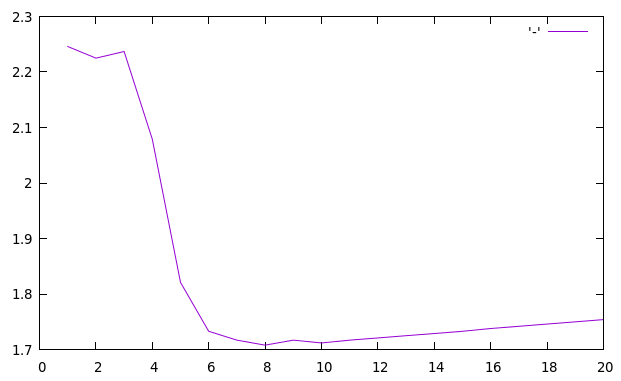
\includegraphics[scale=0.7]{./images/gto_genomic_period.png}
  \caption{\texttt{gto\char`_genomic\char`_period} execution plot.}
  \label{fig:gtoGenomicPeriod}
 \end{figure}
\section{Program gto\char`_genomic\char`_count\char`_bases}
The \texttt{gto\char`_genomic\char`_count\char`_bases} counts the number of bases in a sequence, FASTA or FASTQ files.\\
For help type:
\begin{lstlisting}
./gto_genomic_count_bases -h
\end{lstlisting}
In the following subsections, we explain the input and output parameters.

\subsection*{Input parameters}

The \texttt{gto\char`_genomic\char`_count\char`_bases} program needs two streams for the computation, namely the input and output standard. The input stream is a sequence, FASTA or FASTQ file.\\
The attribution is given according to:
\begin{lstlisting}
Usage: ./gto_genomic_count_bases [options] [[--] args]
   or: ./gto_genomic_count_bases [options]

It counts the number of bases in sequence, FASTA or FASTQ files.

    -h, --help    Show this help message and exit

Basic options
    < input       Input sequence, FASTA or FASTQ file format (stdin)
    > output      Output read information (stdout)

Example: ./gto_genomic_count_bases < input.seq > output

Output example :
File type        : value
Number of bases  : value
Number of a/A    : value
Number of c/C    : value
Number of g/G    : value
Number of t/T    : value
Number of n/N    : value
Number of others : value
\end{lstlisting}
An example of such an input file is:
\begin{lstlisting}
TCTTTACTCGCGCGTTGGAGAAATACAATAGTGCGGCTCTGTCTCCTTATGAAGTCAACAATTTCGCTGGGACTTGCGGC
TCTTTACTCGCGCGTTGGAGAAATACAATAGTGCGGCTCTGTCTCCTTATGAAGTCAACAATTTCGCTGGGACTTGCGGC
GACTTCATCGTGGTCTCTGTCATTATGCGCTCCAACGCATAACTTTGCGCCAGAAGATAGATAGAATGGTGTAAGAAACT
GTAATATATATAATGAACTTCGGCGAGTCTGTGGAGTTTTTGTTGCATTAGAGAGCCAAGAGGTCGGACGTCCTCACGTA
GCCCGAGACGGGCAGGGCGATGGCGACTGAACGGGCTCCATATCACTTTGAGCTTTTATGCTTTCGACTCCTCCAGGAGC
TGAACAACCTTGTTCCCGGCAAAGCCCACTGCGTCATGGAGCTCACGGTCTACATTCATGACTGACTAACCGTAAACTGC
\end{lstlisting}

\subsection*{Output}
The output of the \texttt{gto\char`_genomic\char`_count\char`_bases} program is a report which describes the count of each base in the file, and the file type.\\
Using the input above, an output example of this is:
\begin{lstlisting}
File type        : DNA
Number of bases  : 480
Number of a/A    : 114
Number of c/C    : 116
Number of g/G    : 120
Number of t/T    : 130
Number of n/N    : 0
Number of others : 0
\end{lstlisting}
\section{Program gto\char`_genomic\char`_compressor}
The \texttt{gto\char`_genomic\char`_compressor} is able to provide additional compression gains over several top specific tools, while as an analysis tool, it is able to determine absolute measures, namely for many distance computations, and local measures, such as the information content contained in each element, providing a way to quantify and locate specific genomic events.\\
For help type:
\begin{lstlisting}
./gto_genomic_compressor -h
\end{lstlisting}
In the following subsections, we explain the input and output parameters.

\subsection*{Input parameters}

The \texttt{gto\char`_genomic\char`_compressor} program needs a sequence to compress.\\
The attribution is given according to:
\begin{lstlisting}
SYNOPSIS                                                                
      ./gto_genomic_compressor [OPTION]... -r [FILE] [FILE]:[FILE]:[FILE]:[...]          
                                                                        
SAMPLE                                                                  
      Run Compression         :  ./gto_genomic_compressor -v -l 3 sequence.txt           
      Run Decompression       :  ./gto_genomic_decompressor -v sequence.txt.co             
      Run Information Profile :  ./gto_genomic_compressor -v -l 3 -e sequence.txt        
                                                                        
DESCRIPTION                                                             
      Compress and decompress genomic sequences for storage purposes.   
      Measure an upper bound of the sequences entropy.                  
      Compute information profiles of genomic sequences.                
                                                                        
      -h,  --help                                                       
           usage guide (help menu).                                     
                                                                        
      -V,  --version                                                    
           Display program and version information.                     
                                                                        
      -F,  --force                                                      
           force mode. Overwrites old files.                            
                                                                        
      -v,  --verbose                                                    
           verbose mode (more information).                             
                                                                        
      -x,  --examples                                                   
           show several running examples (parameter examples).          
                                                                        
      -s,  --show-levels                                                
           show pre-computed compression levels (configured parameters).
                                                                        
      -e,  --estimate                                                   
           it creates a file with the extension ".iae" with the       
           respective information content. If the file is FASTA or      
           FASTQ it will only use the "ACGT" (genomic) sequence.      
                                                                        
      -l [NUMBER],  --level [NUMBER]                                    
           Compression level (integer).                                 
           Default level: 5.                                           
           It defines compressibility in balance with computational     
           resources (RAM & time). Use -s for levels perception.        
                                                                        
      -tm [NB_C]:[NB_D]:[NB_I]:[NB_H]:[NB_G]/[NB_S]:[NB_E]:[NB_A]       
           Template of a target context model.                          
           Parameters:                                                  
           [NB_C]: (integer [1;20]) order size of the regular context   
                   model. Higher values use more RAM but, usually, are  
                   related to a better compression score.               
           [NB_D]: (integer [1;5000]) denominator to build alpha, which 
                   is a parameter estimator. Alpha is given by 1/[NB_D].
                   Higher values are usually used with higher [NB_C],   
                   and related to confiant bets. When [NB_D] is one,    
                   the probabilities assume a Laplacian distribution.   
           [NB_I]: (integer {0,1,2}) number to define if a sub-program  
                   which addresses the specific properties of DNA       
                   sequences (Inverted repeats) is used or not. The     
                   number 2 turns ON this sub-program without the       
                   regular context model (only inverted repeats). The   
                   number 1 turns ON the sub-program using at the same  
                   time the regular context model. The number 0 does    
                   not contemple its use (Inverted repeats OFF). The    
                   use of this sub-program increases the necessary time 
                   to compress but it does not affect the RAM.          
           [NB_H]: (integer [1;254]) size of the cache-hash for deeper  
                   context models, namely for [NB_C] > 14. When the     
                   [NB_C] <= 14 use, for example, 1 as a default. The   
                   RAM is highly dependent of this value (higher value  
                   stand for higher RAM).                               
           [NB_G]: (real [0;1)) real number to define gamma. This value 
                   represents the decayment forgetting factor of the    
                   regular context model in definition.                 
           [NB_S]: (integer [0;20]) maximum number of editions allowed  
                   to use a substitutional tolerant model with the same 
                   memory model of the regular context model with       
                   order size equal to [NB_C]. The value 0 stands for   
                   turning the tolerant context model off. When the     
                   model is on, it pauses when the number of editions   
                   is higher that [NB_C], while it is turned on when    
                   a complete match of size [NB_C] is seen again. This  
                   is probabilistic-algorithmic model very usefull to   
                   handle the high substitutional nature of genomic     
                   sequences. When [NB_S] > 0, the compressor used more 
                   processing time, but uses the same RAM and, usually, 
                   achieves a substantial higher compression ratio. The 
                   impact of this model is usually only noticed for     
                   [NB_C] >= 14.                                        
           [NB_E]: (integer [1;5000]) denominator to build alpha for    
                   substitutional tolerant context model. It is         
                   analogous to [NB_D], however to be only used in the  
                   probabilistic model for computing the statistics of  
                   the substitutional tolerant context model.           
           [NB_A]: (real [0;1)) real number to define gamma. This value 
                   represents the decayment forgetting factor of the    
                   substitutional tolerant context model in definition. 
                   Its definition and use is analogus to [NB_G].        
                                                                        
      ... (you may use several target models with custom parameters)    
                                                                        
      -rm [NB_C]:[NB_D]:[NB_I]:[NB_H]:[NB_G]/[NB_S]:[NB_E]:[NB_A]       
           Template of a reference context model.                       
           Use only when -r [FILE] is set (referential compression).    
           Parameters: the same as in -tm.                              
                                                                        
      ... (you may use several reference models with custom parameters) 
                                                                        
      -r [FILE], --reference [FILE]                                     
           Reference sequence filename ("-rm" are trainned here).     
           Example: -r file1.txt.                                       
                                                                        
      [FILE]                                                            
           Input sequence filename (to compress) -- MANDATORY.          
           File(s) to compress (last argument).                         
           For more files use splitting ":" characters.               
           Example: file1.txt:file2.txt:file3.txt.
\end{lstlisting}
In the following example, seventeen DNA sequences are downloaded and the smallest (BuEb) is compressed and decompress. Finally, the uncompressed sequence is compared with the original one to verify that they are the same.
\begin{lstlisting}
wget http://sweet.ua.pt/pratas/datasets/DNACorpus.zip
unzip DNACorpus.zip
cp DNACorpus/BuEb .
../../bin/gto_genomic_compressor -v -l 2 BuEb
../../bin/gto_genomic_decompressor -v BuEb.co 
cmp BuEb BuEb.de -l
\end{lstlisting}
\section{Program gto\char`_genomic\char`_complement}
The \texttt{gto\char`_genomic\char`_complement} replaces the ACGT bases with their complements in a DNA sequence. It works in sequence file formats.\\
For help type:
\begin{lstlisting}
./gto_genomic_complement -h
\end{lstlisting}
In the following subsections, we explain the input and output parameters.

\subsection*{Input parameters}

The \texttt{gto\char`_genomic\char`_complement}  program needs two parameters, namely the input and output standard. The input stream is a sequence file.\\
The attribution is given according to:
\begin{lstlisting}
Usage: ./gto_genomic_complement [options] [[--] args]
   or: ./gto_genomic_complement [options]

It replaces the ACGT bases with their complements in a DNA sequence.
It works in sequence file formats


    -h, --help        Show this help message and exit

Basic options
    < input.seq       Input sequence file (stdin)
    > output.seq      Output sequence file (stdout)

Example: ./gto_genomic_complement < input.seq > output.seq
\end{lstlisting}
An example of such an input file is:
\begin{lstlisting}
TCTTTACTCGCGCGTTGGAGAAATACAATAGTGCGGCTCTGTCTCCTTATGAAGTCAACAATTTCGCTGGGACTTGCGG
CTCTTTACTCGCGCGTTGGAGAAATACAATAGTGCGGCTCTGTCTCCTTATGAAGTCAACAATTTCGCTGGGACTTGCG
GCGACTTCATCGTGGTCTCTGTCATTATGCGCTCCAACGCATAACTTTGCGCCAGAAGATAGATAGAATGGTGTAAGAA
ACTGTAATATATATAATGAACTTCGGCGAGTCTGTGGAGTTTTTGTTGCATTAGAGAGCCAAGAGGTCGGACGTCCTCA
CGTAGCCCGAGACGGGCAGGGCGATGGCGACTGAACGGGCTCCATATCACTTTGAGCTTTTATGCTTTCGACTCCTCCA
GGAGCTGAACAACCTTGTTCCCGGCAAAGCCCACTGCGTCATGGAGCTCACGGTCTACATTCATGACTGACTAACCGTA
AACTGC
\end{lstlisting}

\subsection*{Output}
The output of the \texttt{gto\char`_genomic\char`_complement} program is a group sequence with the ACGT base complements.\\
Using the input above, an output example of this is:
\begin{lstlisting}
AGAAATGAGCGCGCAACCTCTTTATGTTATCACGCCGAGACAGAGGAATACTTCAGTTGTTAAAGCGACCCTGAACGCC
GAGAAATGAGCGCGCAACCTCTTTATGTTATCACGCCGAGACAGAGGAATACTTCAGTTGTTAAAGCGACCCTGAACGC
CGCTGAAGTAGCACCAGAGACAGTAATACGCGAGGTTGCGTATTGAAACGCGGTCTTCTATCTATCTTACCACATTCTT
TGACATTATATATATTACTTGAAGCCGCTCAGACACCTCAAAAACAACGTAATCTCTCGGTTCTCCAGCCTGCAGGAGT
GCATCGGGCTCTGCCCGTCCCGCTACCGCTGACTTGCCCGAGGTATAGTGAAACTCGAAAATACGAAAGCTGAGGAGGT
CCTCGACTTGTTGGAACAAGGGCCGTTTCGGGTGACGCAGTACCTCGAGTGCCAGATGTAAGTACTGACTGATTGGCAT
TTGACG
\end{lstlisting}
\section{Program gto\char`_genomic\char`_reverse}
The \texttt{gto\char`_genomic\char`_reverse} reverses the ACGT bases order for each read in a sequence file.\\
For help type:
\begin{lstlisting}
./gto_genomic_reverse -h
\end{lstlisting}
In the following subsections, we explain the input and output parameters.

\subsection*{Input parameters}

The \texttt{gto\char`_genomic\char`_reverse} program needs two streams for the computation, namely the input and output standard. The input stream is a sequence file.\\
The attribution is given according to:
\begin{lstlisting}
Usage: ./gto_genomic_reverse [options] [[--] args]
   or: ./gto_genomic_reverse [options]

It reverses the ACGT bases order for each read in a sequence file.

    -h, --help        show this help message and exit

Basic options
    < input.seq       Input sequence file (stdin)
    > output.seq      Output sequence file (stdout)

Example: ./gto_genomic_reverse < input.seq > output.seq
\end{lstlisting}
An example of such an input file is:
\begin{lstlisting}
ACAAGACGGCCTCCTGCTGCTGCTGCTCTCCGGGGCCACGGCCCTGGAGGGTCCACCGCTGCCCTGCTGCCATTGTCCCC
GGCCCCACCTAAGGAAAAGCAGCCTCCTGACTTTCCTCGCTTGGGCCGAGACAGCGAGCATATGCAGGAAGCGGCAGGAA
GTGGTTTGAGTGGACCTCCGGGCCCCTCATAGGAGAGGAAGCTCGGGAGGTGGCCAGGCGGCAGGAAGCAGGCCAGTGCC
GCGAATCCGCGCGCCGGGACAGAATCTCCTGCAAAGCCCTGCAGGAACTTCTTCTGGAAGACCTTCTCCACCCCCCCAGC
TAAAACCTCACCCATGAATGCTCACGCAAGTTTAATTACAGACCTGAAACAAGATGCCATTGTCCCCCGGCCTCCTGCTG
CTGCTGCTCTCCGGGGCCACGGCCACCGCTGCCCTGCCCCTGGAGGGTGGCCCCACCGGCCGAGACAGCGAGCATATGCA
GGAAGCGGCAGGAATAAGGAAAAGCAGCCTCCTGACTTTCCTCGCTTGGTGGTTTGAGTGGACCTCCCAGGCCAGTGCCG
GGCCCCTCATAGGAGAGGAAGCTCGGGAGGTGGCCAGGCGGCAGGAAGGCGCACCCCCCCAGCAATCCGCGCGCCGGGAC
AGAATGCCCTGCAGGAACTTCTTCTGGAAGACCTTCTCCTCCTGCAAATAAAACCTCACCCATGAATGCTCACGCAAGTT
TAATTACAGACCTGAA
\end{lstlisting}

\subsection*{Output}
The output of the \texttt{gto\char`_genomic\char`_reverse} program is a group sequence.\\
Using the input above, an output example of this is:
\begin{lstlisting}
AAGTCCAGACATTAATTTGAACGCACTCGTAAGTACCCACTCCAAAATAAACGTCCTCCTCTTCCAGAAGGTCTTCTTCA
AGGACGTCCCGTAAGACAGGGCCGCGCGCCTAACGACCCCCCCACGCGGAAGGACGGCGGACCGGTGGAGGGCTCGAAGG
AGAGGATACTCCCCGGGCCGTGACCGGACCCTCCAGGTGAGTTTGGTGGTTCGCTCCTTTCAGTCCTCCGACGAAAAGGA
ATAAGGACGGCGAAGGACGTATACGAGCGACAGAGCCGGCCACCCCGGTGGGAGGTCCCCGTCCCGTCGCCACCGGCACC
GGGGCCTCTCGTCGTCGTCGTCCTCCGGCCCCCTGTTACCGTAGAACAAAGTCCAGACATTAATTTGAACGCACTCGTAA
GTACCCACTCCAAAATCGACCCCCCCACCTCTTCCAGAAGGTCTTCTTCAAGGACGTCCCGAAACGTCCTCTAAGACAGG
GCCGCGCGCCTAAGCGCCGTGACCGGACGAAGGACGGCGGACCGGTGGAGGGCTCGAAGGAGAGGATACTCCCCGGGCCT
CCAGGTGAGTTTGGTGAAGGACGGCGAAGGACGTATACGAGCGACAGAGCCGGGTTCGCTCCTTTCAGTCCTCCGACGAA
AAGGAATCCACCCCGGCCCCTGTTACCGTCGTCCCGTCGCCACCTGGGAGGTCCCGGCACCGGGGCCTCTCGTCGTCGTC
GTCCTCCGGCAGAACA
\end{lstlisting}
